\documentclass[a4paper,11pt]{article}

\usepackage[english]{babel}
\usepackage[utf8]{inputenc}
\usepackage[vmargin=3.5cm,hmargin=2cm]{geometry}
\usepackage{graphicx}
\usepackage{caption}
\usepackage{subcaption}
\usepackage{amsmath}
\usepackage{mathtools}
\usepackage{fancyhdr}
\usepackage{listings}

\setlength{\footskip}{0cm}
\setlength\parindent{0pt}
\addtolength{\footskip}{0.8cm}
\addtolength{\headsep}{-.5cm}

\title{\bfseries Lab 2.0: \\ Signals and Systems Computations using Matlab\\}
\date{}

\lfoot{}
\cfoot{}
\rfoot{\textbf{Communication Systems} \\ Teresa Algarra Ulierte }

\renewcommand{\headrulewidth}{0.5pt}
\renewcommand{\footrulewidth}{0.5pt}

\begin{document}
\renewcommand\contentsname{\vspace{-1cm}}
\maketitle
\lstset{language=Matlab}

\begin{centering}
    Teresa Algarra Ulierte \\
    Student ID: teresaalgarraulierte \\
    Perm number: 7626872 \\
\end{centering}

\vspace{3cm}

\begin{figure}[!ht]
	\centering
	
\includegraphics[scale = 5]{images/portada.jpeg}
\end{figure}

\newpage

\section{Goal of the lab:}

The goal of this lab is to gain familiarity with computations and plots with Matlab, and to reinforce key concepts in signals and systems.  The questions are chosen to illustrate how we can emulate continuous time operations using the discrete time framework provided by Matlab.

\section{Laboratory assignment:}

\subsection{Functions and Plots:}

To write a function \textit{signalx} that evaluates the following signal at an arbitrary set of points:

\bigskip

\begin{equation}\label{eq:ex1}
    x(t) = 
    \begin{cases} 
      2e^{t+2} & -3 \leq t \leq -1 \\
      2e^{t+2}\cos(2\pi t) & -1 \leq t \leq 4 \\
      0 & else\\
    \end{cases}
\end{equation}

\bigskip

I used a for loop and an if loop:

\bigskip

\begin{lstlisting}
    function [x] = signalx(t)
        N = length(t);                              %Length of the array
        x = zeros(N,1);                             %Creating the vector x
        j = 1;                                      %Iterator for the loop    
        
        for z = t                                   %Check every value of t
            if z < -3                               %First condition
                value = 0;                          %First value
            elseif (z >= -3) && (z <= -1)           %Second condition
                value = 2.*exp(z+2);                %Second value
            elseif (z >= -1) && (z <= 4)            %Third condition
                value = 2.*exp(-z).*cos(2*pi*z);    %Third value
            elseif z > 4                            %Fourth condition
                value = 0;                          %Fourth value
            end                                     %End of the conditions
        
            x(j) = value;                           %Assigning the value to x
            j = j+1;                                %Moving the iterator
        end                                         %End of the loop
    end
\end{lstlisting}

\bigskip

In parts b, c, d and e, I used this function to plot $x(t)$, $x(t-3)$, $x(3-t)$ and $x(2t)$ versus $t$ for $-6\leq t \leq 6$. As a result, I created the following plot: 

\newpage

\begin{figure}[!hp]
    \begin{center}
      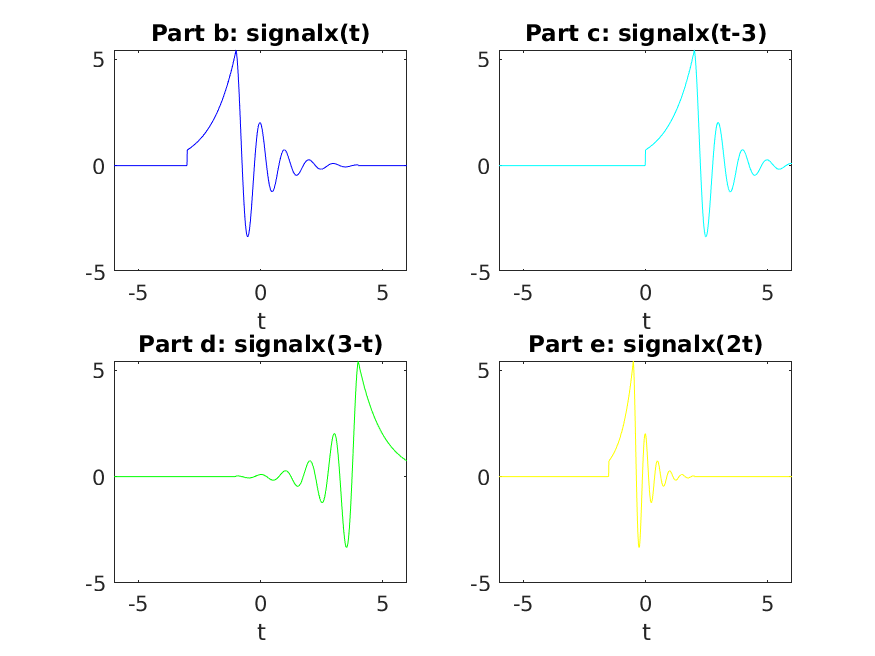
\includegraphics[width=0.9\textwidth]{images/exercice_1.png}
      \captionof{figure}{Exercice 1}
    \end{center}
\end{figure}

\subsection{Convolution:}

For this part, I wrote a Matlab function called \textit{contconv} that computes an approximation to continuous-time convolution. 

\begin{itemize}
    \item Inputs:
    \begin{itemize}
        \item \textbf{x1, x2}: Signals to be convolved.
        \item \textbf{t1, t2}: Starting times for the samples of \textbf{x1} and \textbf{x2} respectively.
        \item \textbf{dt}: Spacing of the samples.
    \end{itemize}
    \item Outputs:
    \begin{itemize}
        \item \textbf{y}: Convolution output.
        \item \textbf{t}: Sampling times for \textbf{y}.
    \end{itemize}
\end{itemize}

\newpage

Therefore, the final function was:

\bigskip

\begin{lstlisting}
    function [y, t] = contconv(x1, x2, t1, t2, dt)
        y=conv(x1,x2)*dt;
        t = (0 : length(y)-1)*dt + t1 + t2;  
    end
\end{lstlisting}

\bigskip

This is a simple script in which I used the built-in convolution MatLab function and adapted it to our sampling rate, that is, \textbf{dt}. Then, I created the time vector knowing that the convolution would start at $t_{0} = t_{1} + t_{2}$ and would finish at $t_{n} = length(y) + t_{1} + t_{2} -1$.

\bigskip

To check that the funtion was working as it should, I convolved two boxes: $3I_{[-2,-1]}(t)$ and $4I_{[1,3]}(t)$. Using the code fragment given in the book, I created the following plot:

\begin{figure}[!hp]
    \begin{center}
      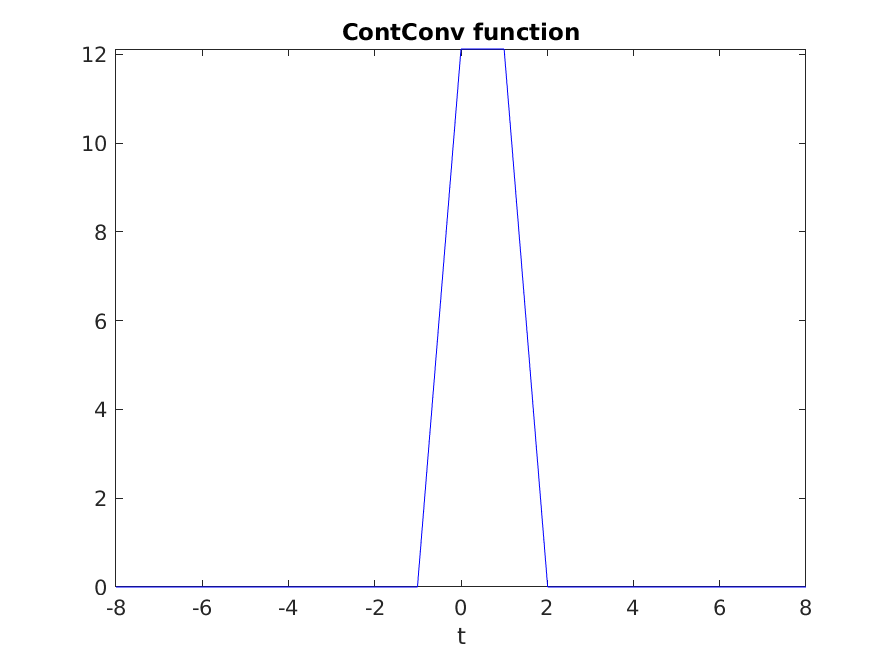
\includegraphics[width=0.9\textwidth]{images/exercice_2.png}
      \captionof{figure}{Exercice 2}
    \end{center}
\end{figure}

\newpage

\subsection{Matched Filter:}

First, I had to plot the signal $u(t) = 2I_{[1,3]}(t) - 3I_{[2,4]}(t)$ and its matched filter, that it, $u*(-t)$. To get $u(t)$, I had to define a time vector $t$ and perform a logic operation. When $t\leq 0$, the result is 1, and when $t > 0$, the result is 0. Doing the same for both limits and multiplying them gives a vector where the 1-values are the intersection of both vectors and, therefore, the desired rectangular funtion. 

\bigskip

\begin{lstlisting}
    dt = 0.01;
    t = -5 : dt : 5;
    u = 2*((t>=1).*(t<=3)) - 3*((t>=2).*(t<=4));
\end{lstlisting}

\bigskip

To get the matched filter, I took the conjugate and flipped it:

\bigskip

\begin{lstlisting}
    w = conj(fliplr(u));
\end{lstlisting}

\bigskip

The plot I generated from these two signals was:

\begin{figure}[!hp]
    \begin{center}
      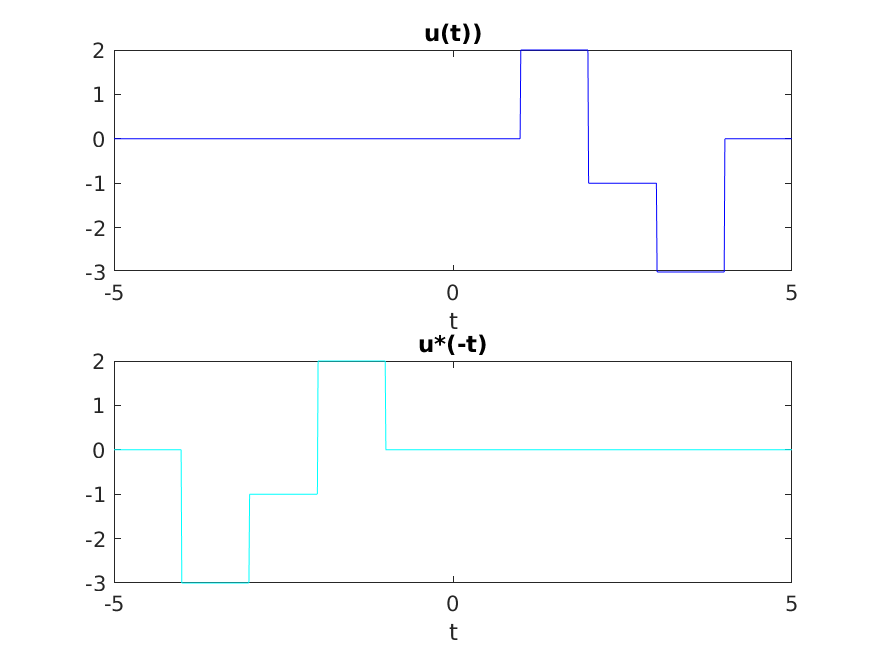
\includegraphics[width=0.9\textwidth]{images/exercice_3a.png}
      \captionof{figure}{Exercice 3.a}
    \end{center}
\end{figure}

\newpage

For the second part of the exercice I had to calculate the convolution of both $u(t)$ and its matched filter and plot the result. The result was:

\begin{figure}[!hp]
    \begin{center}
      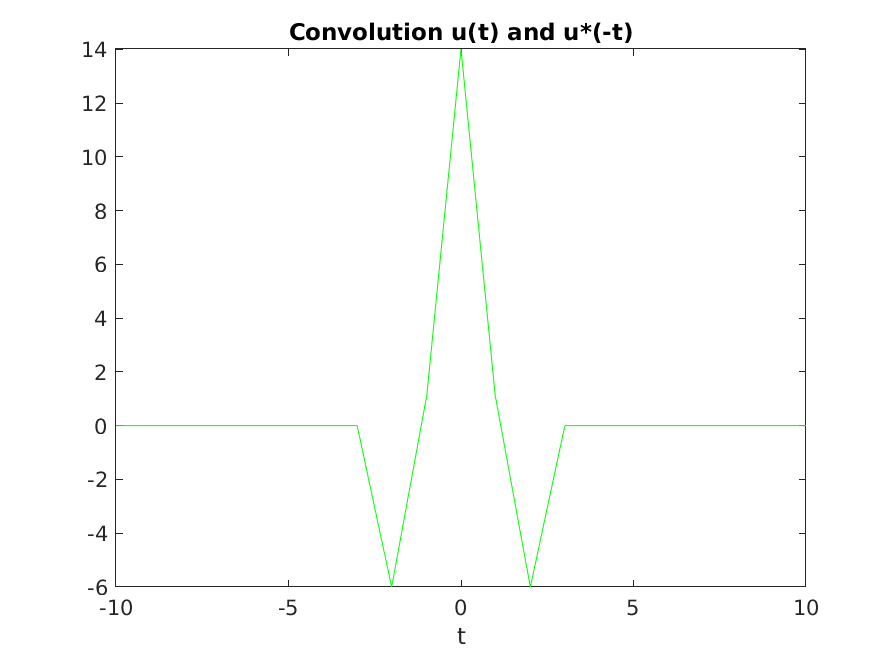
\includegraphics[width=0.9\textwidth]{images/exercice_3b.png}
      \captionof{figure}{Exercice 3.b}
    \end{center}
\end{figure}

The peak is at 0 and it is symmetric with respect to the y-axis.

\bigskip

For the third part of the exercice, I considered a new signal $s(t) = u(t) + jv(t)$ where $u(t)$ is the signal used in parts 1 and 2, and $v(t) = I_{[-1,2]}(t) + 2I_{[0,1]}(t)$. I also considered its matched filter $s_{mf}(t)$. The plot with the real and imaginary parts of both signals is presented below:

\newpage

\begin{figure}[!hp]
    \begin{center}
      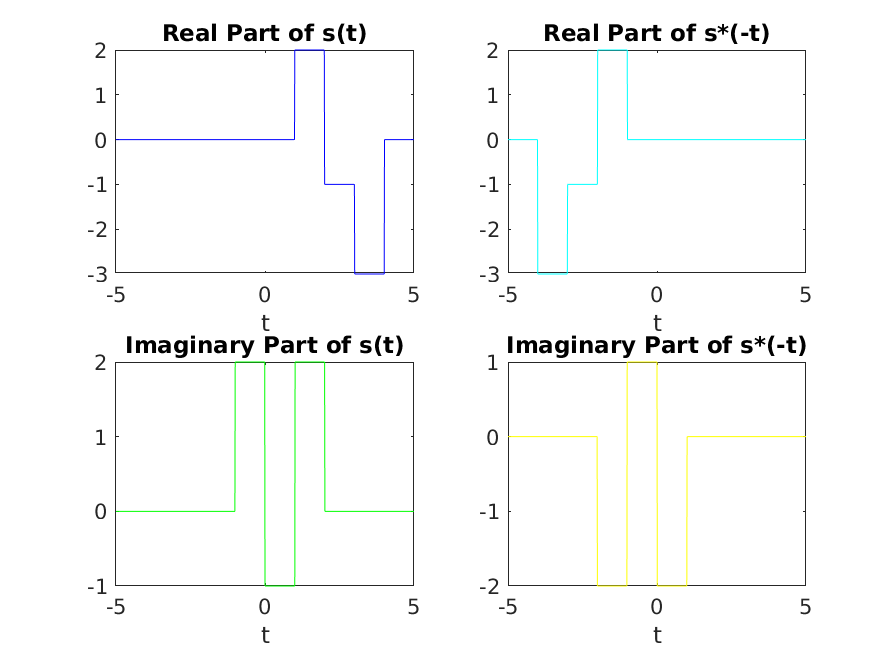
\includegraphics[width=0.7\textwidth]{images/exercice_3c.png}
      \captionof{figure}{Exercice 3.c}
    \end{center}
\end{figure}

The fourth part of the exercice consisted of convolving both $s(t)$ and its matched filter using \textit{contconv}. The required plots were the real part, the imaginary part and the magnitude of the convolution. The result was:

\begin{figure}[!hp]
    \begin{center}
      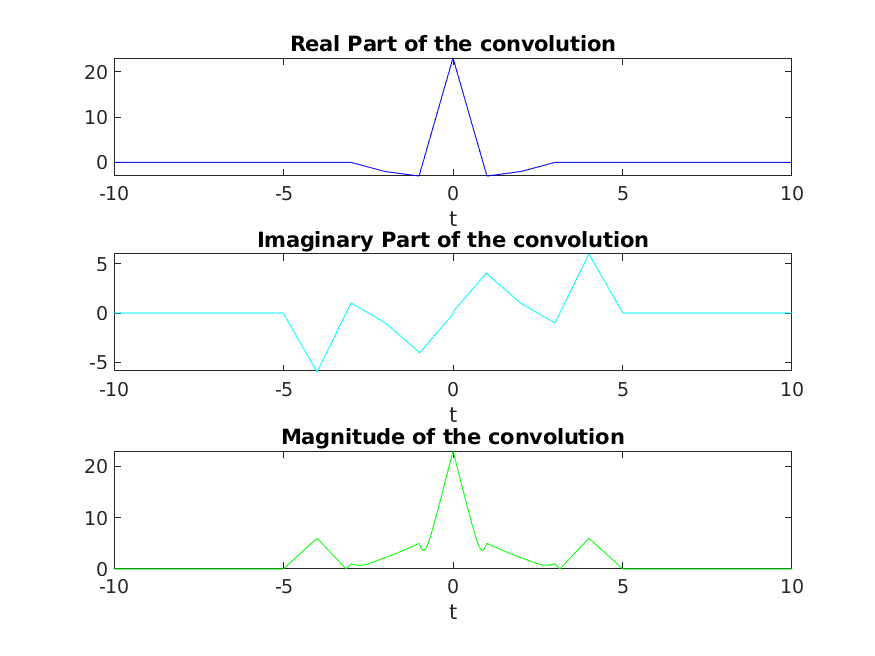
\includegraphics[width=0.7\textwidth]{images/exercice_3d.png}
      \captionof{figure}{Exercice 3.d}
    \end{center}
\end{figure}

For the last plotting part of the exercice, I convolved $s_{1}(t)$ and $s_{mf}(t)$, being $s_{1}(t) = s(t-t_{0})e^{j\theta}$ for $t_{0} = 2$ and $\theta = \frac{\pi}{4}$. Again, I plotted the real part, the imaginary part and the magnitude of the convolution. The result was:

\begin{figure}[!hp]
    \begin{center}
      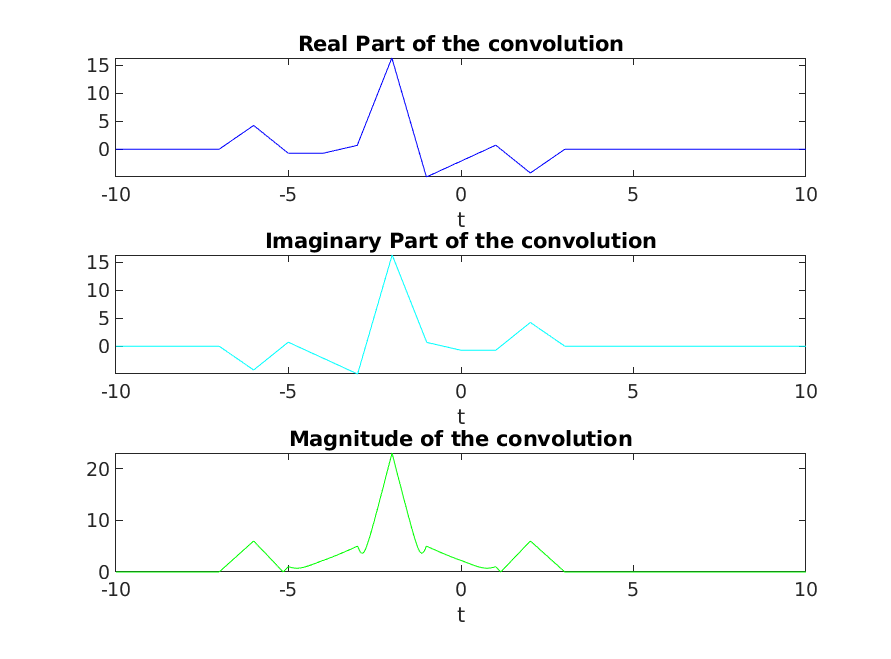
\includegraphics[width=0.7\textwidth]{images/exercice_3e.png}
      \captionof{figure}{Exercice 3.e}
    \end{center}
\end{figure}

This time the peak of the real part and the magnitude of the convolution was not at $t = 0$, but at $t = -t_{0}$, that is, $t = -2$. The peak of the phase is also around -1.6, that is, $-2\frac{\pi}{4}$.

The last question asked for this section was if the output of $s_{1}(t)$ is predictable without knowing the values of $t_{0}$ and $\theta$. My answer is yes because one can estimate how much the peak in the magnitude will move to the left (if $t_{0} > 0$) or to the right (if $t_{0} < 0$). And the same happens with the phase, it will ove to the left (if $\theta > 0$) or to the right (if $\theta < 0$).

\subsection{Fourier Transform:}

For this part of the lab I used the function \textit{contFT} given in the book. I calculated the transform of $s(t) = 3\sinc (2t-3)$ where the sampling rate was $16MHz$ $(dt = \frac{1}{16\times 10^{6}})$ and the desired frequency resolution was $1 KHz$. I calculated the magnitude and the phase of the resulting FT. For that, I used the following piece of code:

\bigskip

\begin{lstlisting}
    dt = 1/(16e6);                          %Sample spacing
    df_i = 1e3;                             %Desired frequency resolution
    t = -8e-6 : dt : 8e-6;                  %Time vector
    s = 3 * sinc(2*t*1e6 - 3);              %Input signal
    [X, f, ~] = contFT(s,t(1),dt,df_i);     %Given funtion
    X_ma = abs(X);                          %Magnitude of the FT
    X_ph = angle(X);                        %Phase of the FT
\end{lstlisting}

\bigskip

The final plots were:

\begin{figure}[!hp]
    \begin{center}
      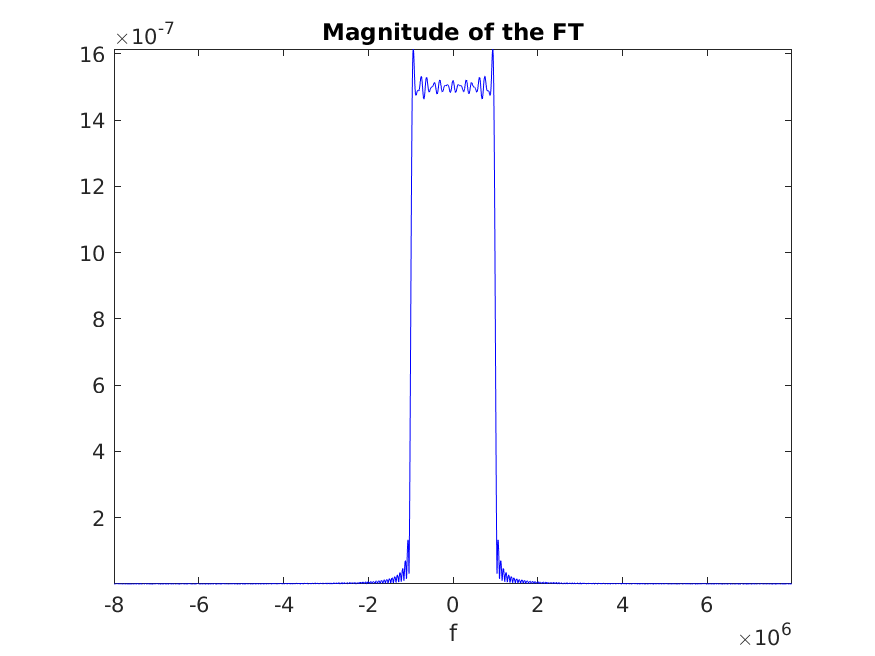
\includegraphics[width=0.7\textwidth]{images/exercice_4a.png}
      \captionof{figure}{Exercice 4.a}
    \end{center}
\end{figure}

\begin{figure}[!hp]
    \begin{center}
      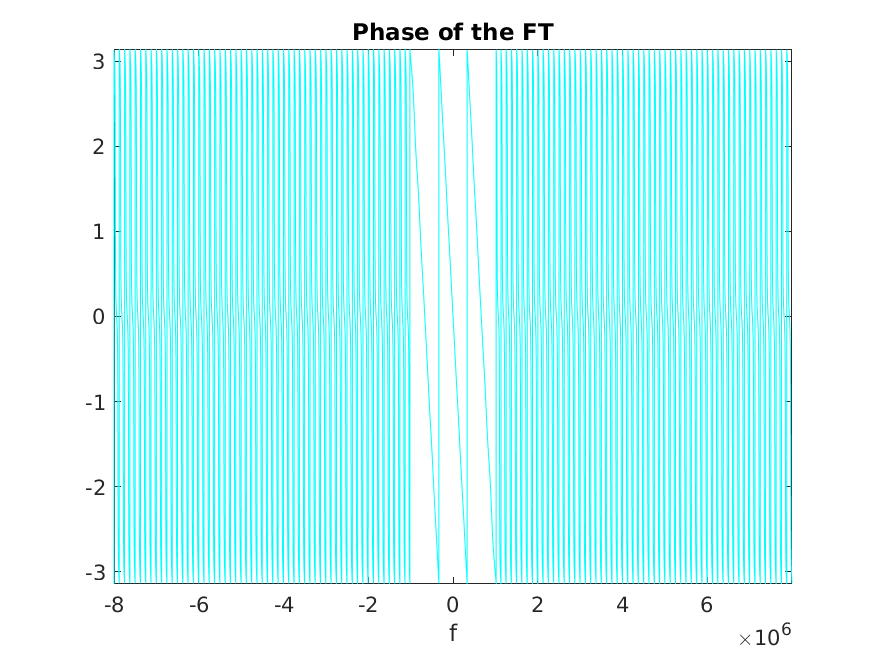
\includegraphics[width=0.7\textwidth]{images/exercice_4b.png}
      \captionof{figure}{Exercice 4.b}
    \end{center}
\end{figure}

As one can see, the phase only has meaning between $-1kHz$ and $1kHz$.

\subsection{Matched Filter in Frequency Domain:}

For this last part, I considered the signal $s(t)$ from section 3. Using milliseconds as time unit and a desired frequency resolution of $1Hz$, I calculated de FT $S(f)$. The magnitude was:

\begin{figure}[!hp]
    \begin{center}
      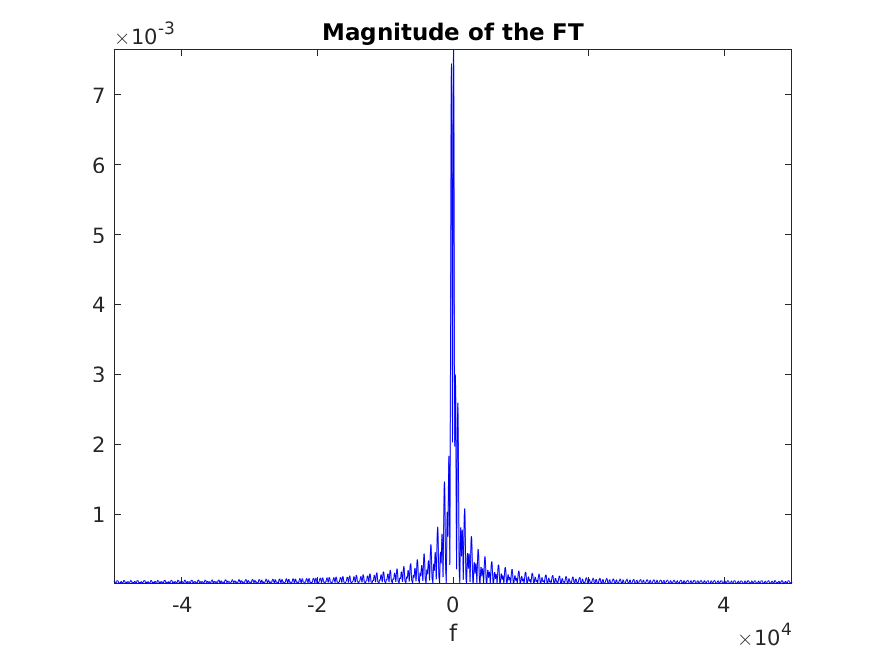
\includegraphics[width=0.65\textwidth]{images/exercice_5a.png}
      \captionof{figure}{Exercice 5.a}
    \end{center}
\end{figure}

By zooming in, one can see the plot in more detail:

\begin{figure}[!hp]
    \begin{center}
      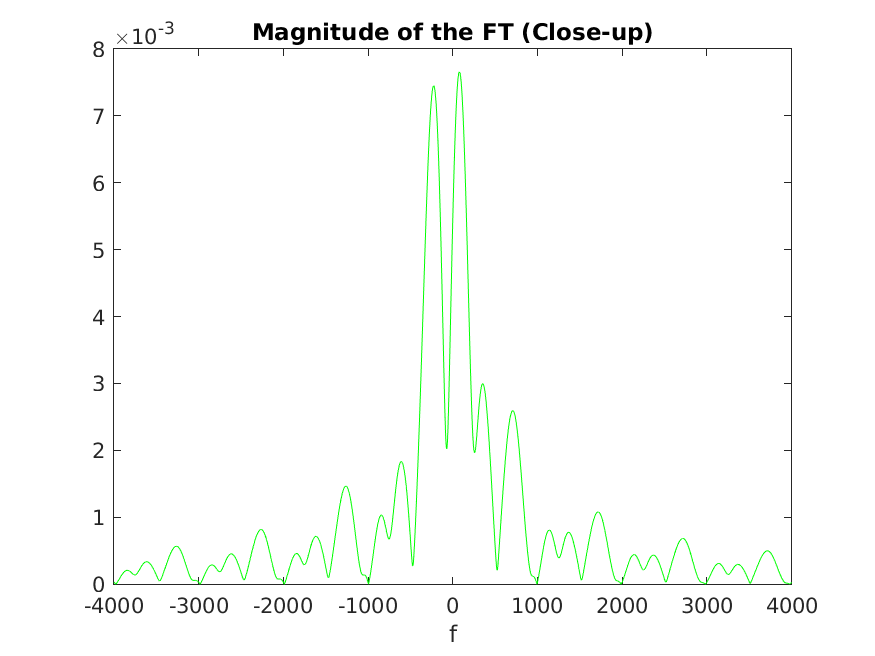
\includegraphics[width=0.65\textwidth]{images/exercice_5a_c.png}
      \captionof{figure}{Exercice 5.a}
    \end{center}
\end{figure}

\newpage

I did the convolution of $s(t)$ and its matched filter $s_{mf}(t)$ followed by the FT of the result:

\bigskip

\begin{lstlisting}
    u = 2* ¡((t>=1e-3).*(t<=3e-3)) - 3*((t>=2e-3).*(t<=4e-3));	%Given signal
    v = ((t>=-1e-3).*(t<=2e-3)) + 2*((t>=0).*(t<=1e-3));        %Given signal
    s = u + 1i*v;                           %Total signal
    g = fliplr(conj(s));                    %Match filter
    [h,y]= contconv(s,g,t(1),t(1),dt);      %Convolution
    [H,k,~] = contFT(h,y(1),dt,df_i);       %Given funtion
    H_ma = abs(H);                          %Magnitude of the FT
    X2 = abs(X).^2;                         %Magnitude square of X
\end{lstlisting}

\bigskip

I also plotted the magnitude $|S(f)|^2$ to see that they are indeed equal.

\begin{figure}[!hp]
    \begin{center}
      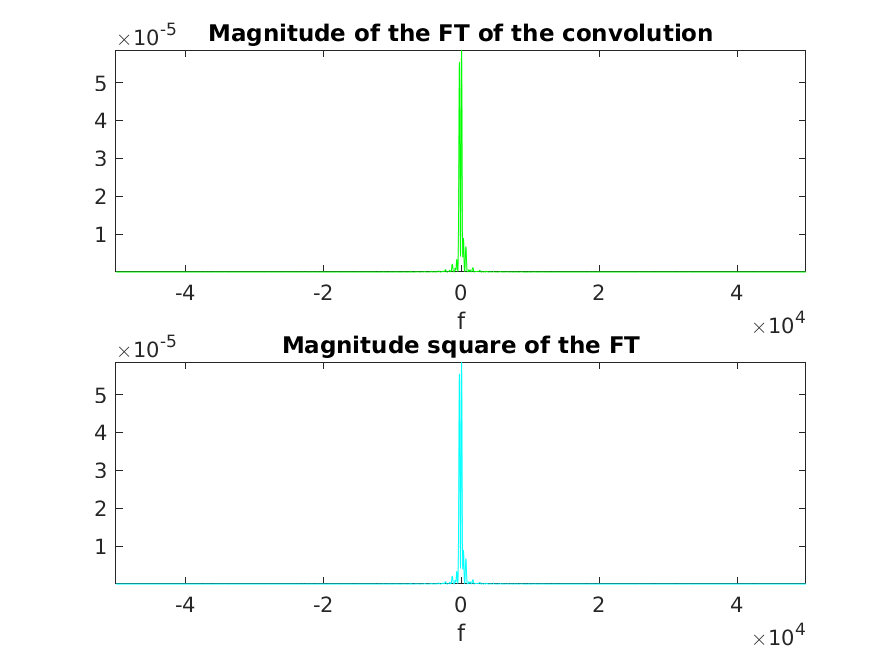
\includegraphics[width=0.9\textwidth]{images/exercice_5b.png}
      \captionof{figure}{Exercice 5.b}
    \end{center}
\end{figure}

\newpage

By zooming in, one can see the plot in more detail:

\begin{figure}[!hp]
    \begin{center}
      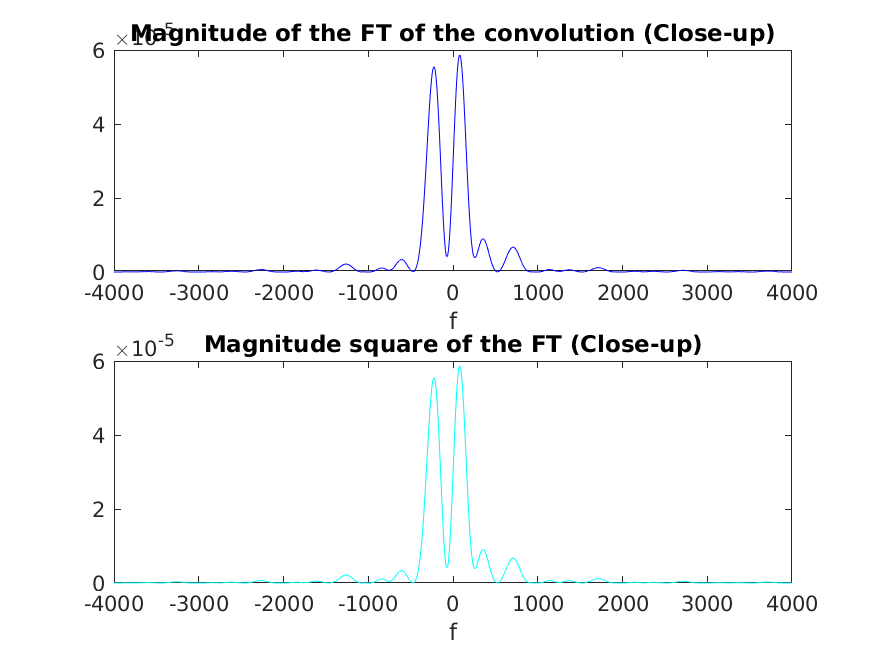
\includegraphics[width=0.65\textwidth]{images/exercice_5b_c.png}
      \captionof{figure}{Exercice 5.b}
    \end{center}
\end{figure}

Lastly, I plotted the phase of the FT above:

\begin{figure}[!hp]
    \begin{center}
      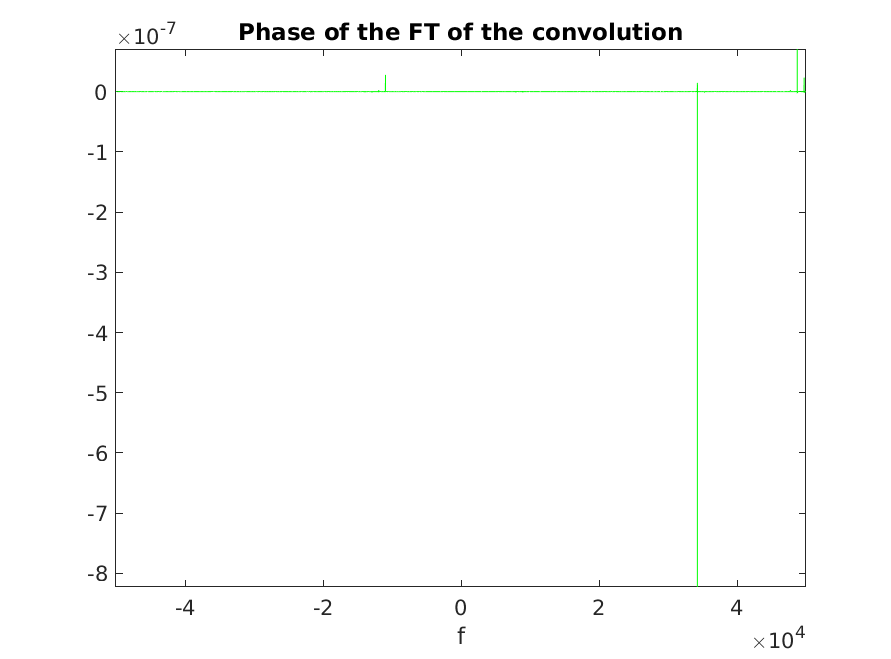
\includegraphics[width=0.65\textwidth]{images/exercice_5c.png}
      \captionof{figure}{Exercice 5.c}
    \end{center}
\end{figure}

\newpage

By focusing on the scale, one can see that all those lines are small numerical errors. By zooming out, one can see the that the phase is 0:


\begin{figure}[!hp]
    \begin{center}
      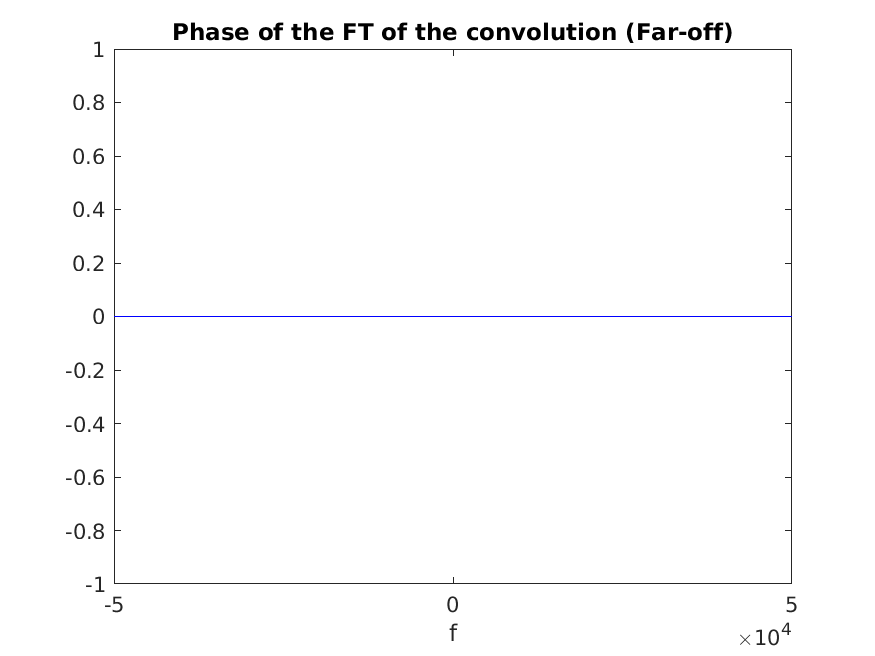
\includegraphics[width=0.9\textwidth]{images/exercice_5c_f.png}
      \captionof{figure}{Exercice 5.c}
    \end{center}
\end{figure}

\section{Conclusion:}

In this lab I got to work with all the functions that we will use during the quarter. In the beggining it was a bit difficult to work with vectors and arrays, but after the second part of the lab everything was easier, so I think I am ready to continue with the rest of the labs.

\vspace{4cm}

\end{document}

